\documentclass[a4paper]{arrowhead}

\usepackage[yyyymmdd]{datetime}
\usepackage{etoolbox}
\usepackage[utf8]{inputenc}
\usepackage{multirow}

\renewcommand{\dateseparator}{-}

%% Special references
\newcommand{\scref}[2]{{\textcolor{ArrowheadBlue}{\hyperref[sec:services:consumed:#1]{#2}}}}
\newcommand{\scdef}[2]{{\textcolor{ArrowheadBlue}{#2\label{sec:services:consumed:#1}}}}
\newcommand{\spref}[2]{{\textcolor{ArrowheadBlue}{\hyperref[sec:services:produced:#1]{#2}}}}
\newcommand{\spdef}[2]{{\textcolor{ArrowheadBlue}{#2\label{sec:services:produced:#1}}}}
%%

\begin{document}

%% Arrowhead Document Properties
\ArrowheadTitle{ServiceRegistry}
\ArrowheadType{System Design Description}
\ArrowheadTypeShort{SysDD}
\ArrowheadVersion{4.3.0}
\ArrowheadDate{\today}
\ArrowheadAuthor{Szvetlin Tanyi}
\ArrowheadStatus{RELEASE}
\ArrowheadContact{szvetlin@aitia.ai}
\ArrowheadFooter{\href{www.arrowhead.eu}{www.arrowhead.eu}}
\ArrowheadSetup
%%

%% Front Page
\begin{center}
  \vspace*{1cm}
  \huge{\arrowtitle}

  \vspace*{0.2cm}
  \LARGE{\arrowtype}
  \vspace*{1cm}
  \vspace*{\fill}

  % Front Page Image
  %\includegraphics{figures/TODO}

  \vspace*{1cm}
  \vspace*{\fill}

  % Front Page Abstract
  \begin{abstract}
    This document describes the Service Registry core system of the Eclipse Arrowhead Framework. This core system takes responsibility for managing the offered services of all systems.
  \end{abstract}

  \vspace*{1cm}

  \scriptsize
  \begin{tabularx}{\textwidth}{l X}
    \raisebox{-0.5\height}{
\includegraphics[width=2cm]{figures/artemis_logo}} & {ARTEMIS Innovation Pilot Project: Arrowhead\newline
    THEME [SP1-JTI-ARTEMIS-2012-AIPP4 SP1-JTI-ARTEMIS-2012-AIPP6]\newline
    [Production and Energy System Automation Intelligent-Built environment and urban infrastructure for sustainable and friendly cities]}
  \end{tabularx}
  \vspace*{-0.2cm}
\end{center}
\newpage
%%

%% Table of Contents
\tableofcontents
\newpage
%%

\section{Overview}
\label{sec:overview}

This document describes the Eclipse Arrowhead  ServiceRegistry system,
which exists to enable service discovery in a Eclipse Arrowhead Local Cloud (LC).  Examples of such interactions is a provider system
  offering some kind of Eclipse Arrowhead service for use by other systems in the LC. 

This Core System provides a database, which stores information related
to the currently actively offered Services within the Local Cloud. The
primary use case situations are indicated in Figure \ref{fig:Use_case_ServiceRegistry}

\begin{figure}[ht!]
  \centering
  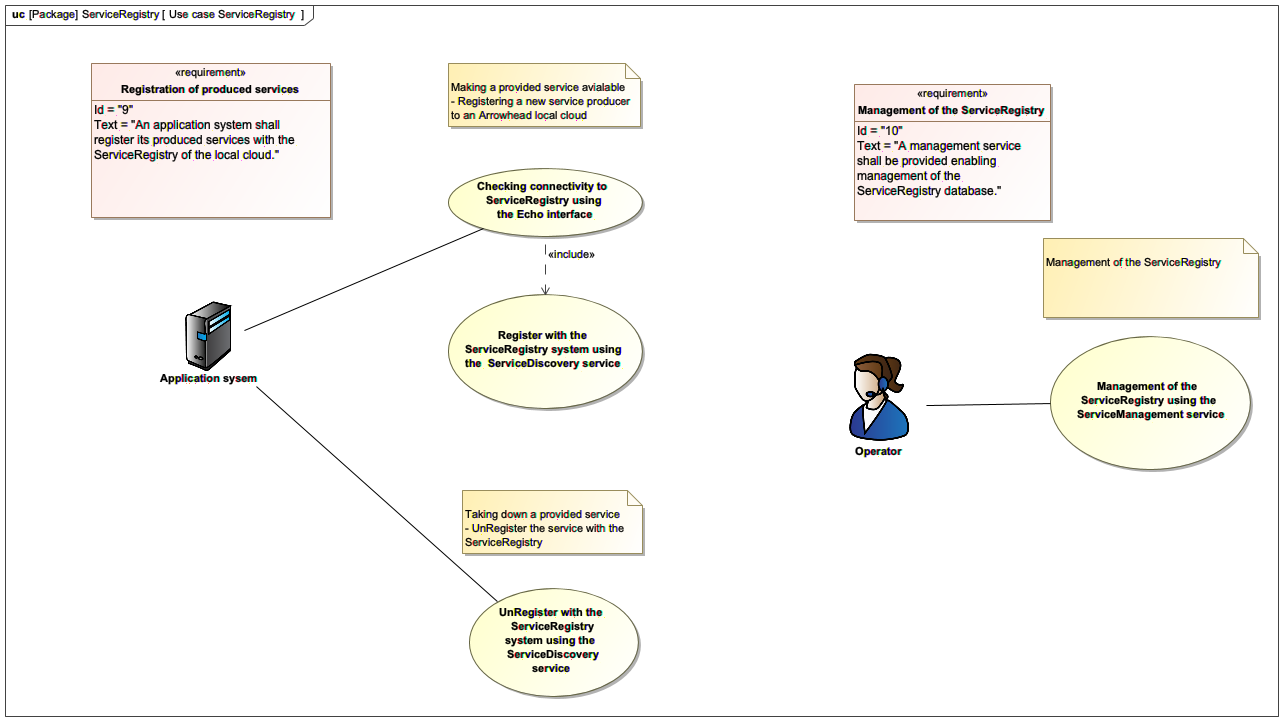
\includegraphics[width=\textwidth]{figures/Use_case_ServiceRegistry}
  \caption{Use case diagram of the ServiceRegistry interaction with
    application systems and operators. }
  \label{fig:Use_case_ServiceRegistry}
\end{figure}

The purpose of this System is therefore to allow:
\begin{itemize}
\item Application Systems to register what Services they offer at the moment, making this announcement available to other Application Systems on the network.
\item They are also allowed to remove or update their entries when it is necessary.
\item  All Application Systems can utilize the lookup functionality of the Registry to find Public Core System Service offerings in the network, otherwise the Orchestrator has to be used.
\end{itemize}




\begin{figure}[t!]
  \centering 
  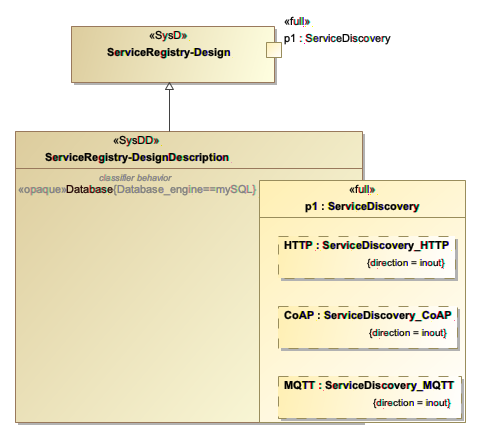
\includegraphics[width=0.8\textwidth]{figures/ServiceRegistry_SysDD}
  \caption{A SysML block description diagram of the Eclipse Arrowhead
    ServiceRegsitry system. v4.3.0 only support HTTP/JSON/TLS while
    the upcoming v4.4.0 will support CoAP/JSON/TLS and MQTT/JSON/TLS
    in addition.}
  \label{fig:ServiceRegistrySysDD}
\end{figure}
%

However, it is worth noting, that within this generation the lookup functionality of Services is integrated within the “orchestration process”. Therefore, in the primary scenario, when an Application System is looking for a Service to consume, it shall ask the Orchestrator System via the Orchestration Service to locate one or more suitable Service Providers and help establish the connection based on metadata submitted in the request. Direct lookups from Application Systems within the network is not advised in this generation, due to security reasons.

However, the lookup of other Application Systems and Services directly is not within the primary use, since access will not be given without the Authorization JWT (JSON Web Token). The use of the TokenGeneration is restricted to the Orchestrator for general System accountability reasons.

The v4.3.0 only supports the HTTP protocol, JSON encoding and TLS
payload protection. For v4.4.0 both CoAP and MQTT will be supported as
well, see Figure \ref{fig:ServiceRegistrySysDD}.
%
%


\section{System Role}
\label{sec:role}

This System only provides one Core Service the \textbf{Service
  Discovery}. 


There are two use case scenarios connected to the Service Registry.
\begin{itemize}
    \item Service registration, de-registration
    \item Service Registry querying (lookup)
\end{itemize}

The register interface is used to register services. The services will contain various metadata as well as a physical endpoint. The various parameters are representing the endpoint information that should be registered.

The unregister interface is used to unregister service instances that were previously registered in the Registry. The instance parameter is representing the endpoint information that should be removed.

The query interface is used to find and translate a symbolic service name into a physical endpoint, for example an IP address and a port. The query parameter is used to request a subset of all the registered services fulfilling the demand of the user of the service. The returned listing contains service endpoints that have been fulfilling the query.

There is another functionality that does not bound to any Services,
just an internal part of the Service Registry. There are two optional
cleanup tasks within the Service Registry, which can be used to remove
old, inactive service offerings. The first task is based on pinging
the service provider and if the provider does not respond to the ping,
its offered services will be deleted. The second task is based on a
feature, called “Time to Live”. Service providers upon registration
can provide a timestamp called “end\_of\_validity” number, which
specifies how long the service will be offered by the provider, making
the service de-registrations unnecessary, if this task is active. The
task is used to remove expired services. The third task is using a
feature called "Heartbeat" (Not yet implemented - for time line see Roadmap), where the Service provider periodically signals to the Service Registry that it is still alive. When it misses it will be removed. All of these internal tasks can be configured in the application.properties file.

\section{Services}
\label{sec:services}


\subsection{Consumed Services}

None.

\subsection{Provided Services}

\subsubsection{\spdef{ServiceDiscovery}{ServiceDiscovery}}

This service is provided to allow other systems to \textbf{Register}
and to \textbf{Unregister} their services, and to \textbf{Query}
public services. In addition the service can Echo that its alive.

\section{Security}
\label{sec:security}

This System can be secured via the HTTPS protocol. If it is started in secure mode, it verifies whether the Application System possesses a proper X.509 identity certificate and whether that certificate is Arrowhead compliant in its' making. This certificate structure and creation guidelines ensure:

\begin{itemize}
    \item Application System is properly bootstrapped into the Local Cloud
    \item The Application System indeed belongs to this Local Cloud
    \item The Application System then automatically has the right to register its Services in the Registry.
   
\end{itemize}

 If these criteria are met, the Application System’s registration or removal message is processed. An Application System can only delete or alter entries that contain the Application System as the Service Provider in the entry.



\newpage

\bibliographystyle{IEEEtran}
\bibliography{bibliography}

\newpage

\section{Revision History}
\subsection{Amendments}

\noindent\begin{tabularx}{\textwidth}{| p{1cm} | p{3cm} | p{2cm} | X | p{4cm} |} \hline
\rowcolor{gray!33} No. & Date & Version & Subject of Amendments & Author \\ \hline

1 & 2020-12-05 & 4.3.0 &  & Tanyi Szvetlin \\ \hline
1 & 2021-01-18 & 4.3.0 & & Jerker Delsing \\ \hline

\end{tabularx}

\subsection{Quality Assurance}

\noindent\begin{tabularx}{\textwidth}{| p{1cm} | p{3cm} | p{2cm} | X |} \hline
\rowcolor{gray!33} No. & Date & Version & Approved by \\ \hline

1 & 2021-01-18 & 4.3.0 & Jerker Delsing \\ \hline

\end{tabularx}

\end{document}